\chapter{TINJAUAN PUSTAKA}
\label{chap:tinjauanpustaka}

% Ubah bagian-bagian berikut dengan isi dari tinjauan pustaka

Demi mendukung penelitian ini, dibutuhkan beberapa teori penunjang sebagai bahan acuan dan referensi. Dengan demikian penelitian ini menjadi lebih terarah.

\section{Convolutional Neural Network}
\label{sec:cnn}

% Contoh input gambar
\begin{figure}[ht]
	\centering
	
	% Ubah dengan nama file gambar dan ukuran yang akan digunakan
	\includegraphics[width=0.7\columnwidth]{gambar/kuda-kudaan.jpeg}
	
	% Ubah dengan keterangan gambar yang diinginkan
	\caption{Seorang anak sedang menaiki kuda mainan \citep{cit:kuda}}
	\label{fig:kudakudaan}
\end{figure}

\emph{Convolutional Neural Network (CNN)} adalah salah satu jenis neural network yang biasa digunakan pada data image \cite{cit:cnn}. CNN bisa digunakan untuk mendeteksi dan mengenali object pada sebuah image. CNN adalah sebuah teknik yang terinspirasi dari cara mamalia — manusia, menghasilkan persepsi visual seperti gambar \ref{fig:kudakudaan} diatas.

Secara garis besar Convolutional Neural Network (CNN) tidak jauh berbeda dengan neural network biasanya. CNN terdiri dari neuron yang memiliki weight, bias dan activation function.

\subsection{Cara Kerja CNN}
Secara garis besarnya, CNN memanfaatkan proses konvolusi dengan menggerakan sebuah kernel konvolusi \textit{(filter)} berukuran tertentu ke sebuah gambar, komputer mendapatkan informasi representatif baru dari hasil perkalian bagian gambar tersebut dengan filter yang digunakan.

\begin{enumerate}
	\item \textbf{Memecah gambar menjadi gambar yang lebih kecil yang tumpang tindih}
	
	Dari gambar seorang anak kecil yang menaiki kuda mainan \ref{fig:kudakudaan}, hasil dari proses konvolusi dapat diilustrasikan sebagai berikut ini:
	
	\begin{figure}[ht]
		\centering
		
		% Ubah dengan nama file gambar dan ukuran yang akan digunakan
		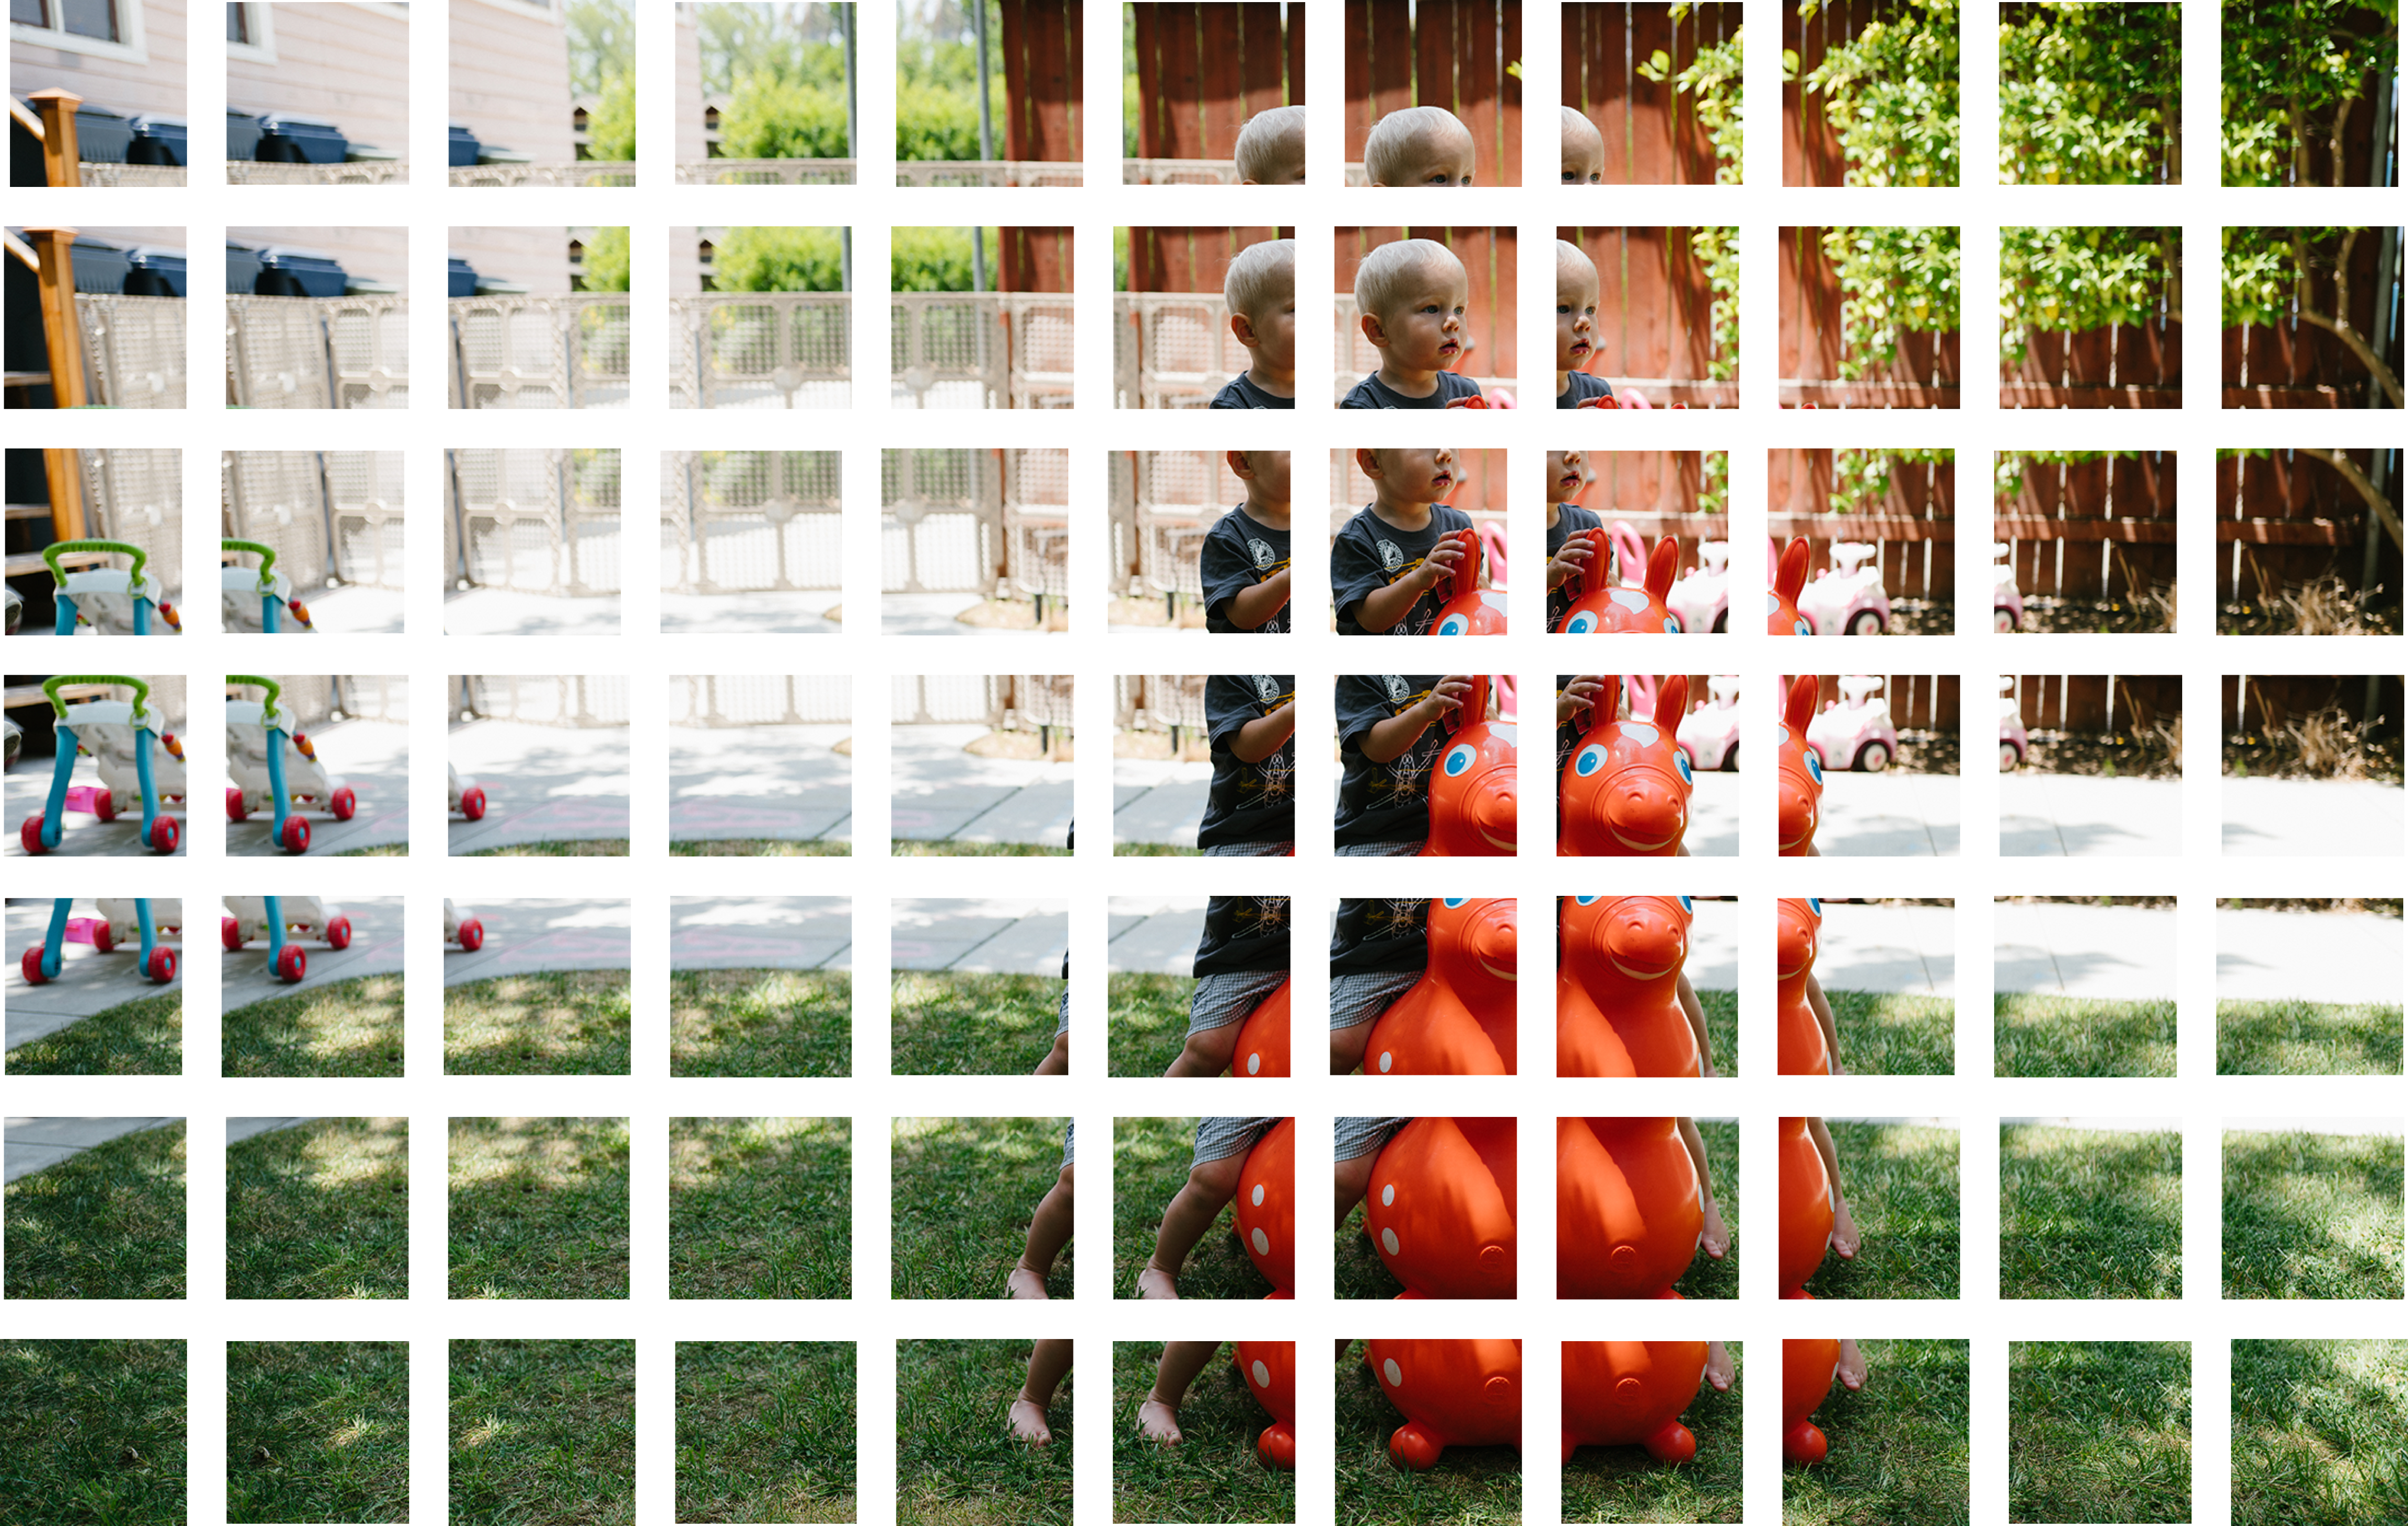
\includegraphics[width=0.7\columnwidth]{gambar/pecahkuda.png}
		
		% Ubah dengan keterangan gambar yang diinginkan
		\caption{Convolution Filter \citep{cit:kuda}}
		\label{fig:kudapecah}
	\end{figure}

	\item \textbf{Memasukkan setiap gambar yang lebih kecil ke small neural network}
	
	Setiap gambar kecil dari hasil konvolusi tersebut kemudian dijadikan input untuk menghasilkan sebuah representasi fitur. Hal ini memberikan CNN kemampuan mengenali sebuah objek, dimanapun posisi objek tersebut muncul pada sebuah gambar.
	
	\begin{figure}[ht]
		\centering
		
		% Ubah dengan nama file gambar dan ukuran yang akan digunakan
		\includegraphics[width=0.7\columnwidth]{gambar/singletile.png}
		
		% Ubah dengan keterangan gambar yang diinginkan
		\caption{Single Tile Processing \citep{cit:kuda}}
		\label{fig:singletile}
	\end{figure}
	
	Proses ini dilakukan untuk semua bagian dari masing-masing gambar kecilnya, dengan menggunakan filter yang sama. Dengan kata lain, setiap bagian gambar akan memiliki faktor pengali yang sama, atau dalam konteks neural network disebut sebagai weights sharing. Jika ada sesuatu yang tampak menarik di setiap gambarnya, maka akan ditandai bagian itu sebagai object of interest.
	
	\item \textbf{Menyimpan hasil dari masing-masing gambar kecil ke dalam array baru}
	
	Hasil dari proses sebelumnya disatukan dan dimasukkan ke dalam array baru, seperti yang dapat di lihat pada gambar \ref{fig:outputarray}.
	
		\begin{figure}[ht]
		\centering
		
		% Ubah dengan nama file gambar dan ukuran yang akan digunakan
		\includegraphics[width=0.7\columnwidth]{gambar/outputarray.png}
		
		% Ubah dengan keterangan gambar yang diinginkan
		\caption{Overall Tile Processing \citep{cit:kuda}}
		\label{fig:outputarray}
	\end{figure}
	
	\item \textit{\textbf{Downsampling}}
	
	Pada langkah 3, array masih terlalu besar yang mana jumlah parameternya akan terlalu banyak untuk di proses dan mengakibatkan penggunaan resource yang terlalu besar, maka dari itu ukuran array tersebut perlu diperkecil. Untuk mengecilkan ukuran array nya digunakan downsampling yang penggunaannya dinamakan max pooling atau mengambil nilai pixel terbesar di setiap pooling kernel. Dengan begitu, sekalipun mengurangi jumlah parameter, informasi terpenting dari bagian tersebut tetap diambil.
	
	\begin{figure}[ht]
		\centering
		
		% Ubah dengan nama file gambar dan ukuran yang akan digunakan
		\includegraphics[width=0.9\columnwidth]{gambar/maxpooling.png}
		
		% Ubah dengan keterangan gambar yang diinginkan
		\caption{\emph{Max Pooling Downsampling} \citep{cit:kuda}}
		\label{fig:maxpooling}
	\end{figure}
	
\end{enumerate}


% Contoh input gambar
\begin{figure}[ht]
  \centering

  % Ubah dengan nama file gambar dan ukuran yang akan digunakan
  \includegraphics[width=0.9\columnwidth]{gambar/cnn.jpeg}

  % Ubah dengan keterangan gambar yang diinginkan
  \caption{\emph{Convolutional Neural Network} \citep{cit:cnn}}
  \label{fig:cnn}
\end{figure}

Berdasarkan Gambar \ref{fig:cnn}, CNN dengan input awal balok tiga dimensi akan ditransformasikan menjadi output tiga dimensi dengan beberapa fungsi diferensiasi yang memiliki atau tidak memiliki parameter. CNN membentuk neuron-neuronnya ke dalam tiga dimensi (panjang, lebar, dan tinggi) dalam sebuah lapisan.

CNN Terdiri atas dua bagian utama, yaitu Feature Learning dan Classification. masing masing bagian dapat dijelaskan sebagai berikut:

\subsection{Feature learning}
\label{subsec:featurelearning}

Lapisan-lapisan yang terdapat dalam Feature Learning berguna untuk mentranslasikan suatu input menjadi menjadi \emph{features} berdasarkan ciri dari input tersebut yang berbentuk angka-angka dalam vektor. Lapisan ekstraksi fitur ini terdiri dari Convolutional Layer dan Pooling Layer.

\begin{enumerate}
	\item \textbf{\textit{Convolutional Layer}} akan menghitung output dari neuron yang terhubung ke daerah lokal dalam input, masing-masing menghitung produk titik antara bobot mereka dan wilayah kecil yang terhubung ke dalam volume input.
	
	\item \textbf{\textit{Rectified Linear Unit (ReLU)}} akan menghilangkan vanishing gradient dengan cara menerapkan fungsi aktivasi elemen sebagai:
	\begin{equation}
		\label{eq:relu} f(x) = max(0, x)
	\end{equation}
	alias aktivasi elemen akan dilakukan saat berada di ambang batas 0.
	
	Kelebihan dalam penggunaan ReLU diantaranya sebagai berikut :
	\begin{itemize}
		\item Bisa mempercepat gradien stokastik dibandingkan dengan fungsi \textit{sigmoid} / \textit{tanh} karena ReLU berbentuk linear
		\item Tidak menggunakan operasi eksponensial seperti \textit{sigmoid} / \textit{tanh}, sehingga bisa melakukan dengan pembuatan matriks aktivasi saat ambang batas berada pada nilai 0
	\end{itemize}
	
	Sedangkan Kekurangan dalam penggunaan ReLU adalah:
	\begin{itemize}
		\item ReLU bisa rapuh saat masa training dan mati karena gradien besar yang mengalir melalui ReLU menyebabkan update bobot, sehingga neuron tidak aktif pada datapoint lagi. Jika ini terjadi, maka gradien yang mengalir melalui unit akan selamanya nol dari titik itu. Artinya, unit ReLU dapat mati secara ireversibel selama pelatihan karena mereka dapat melumpuhkan data manifold. Misalnya, Anda mungkin menemukan bahwa sebanyak 40\% dari jaringan Anda dapat “mati” (yaitu neuron yang tidak pernah aktif di seluruh dataset pelatihan) jika tingkat pembelajaran ditetapkan terlalu tinggi. Dengan pengaturan tingkat pembelajaran yang tepat, ini lebih jarang menjadi masalah
	\end{itemize}
	
\end{enumerate}

\section{Gravitasi}
\label{sec:gravitasi}

Gravitasi merupakan \lipsum[1]

\subsection{Hukum Newton}
\label{subsec:hukumnewton}

Newton \citep{newton1687} pernah merumuskan bahwa \lipsum[1]
Kemudian menjadi persamaan seperti pada persamaan \ref{eq:hukumpertamanewton}.

% Contoh pembuatan persamaan
\begin{equation}
  \label{eq:hukumpertamanewton}
  \sum \mathbf{F} = 0\; \Leftrightarrow\; \frac{\mathrm{d} \mathbf{v} }{\mathrm{d}t} = 0.
\end{equation}

\subsection{Anti Gravitasi}
\label{subsec:antigravitasi}

Anti gravitasi merupakan \lipsum[1]
